% Talk about target complementarity?
\chapter{WIMP Direct detection}\label{chapter:direct}
\lhead{\emph{WIMP Direct detection}}

In this Chapter we introduce the theoretical framework needed to predict signals in WIMP direct detection experiments. We begin in Sec.~\ref{sec:direct_WIMPnucleus} with the particle physics input: the WIMP-nucleus interaction and the derivation of the elastic scattering event rate. In Sec.~\ref{sec:direct_MW} we describe the astrophysical input including the local dark matter density and velocity distribution; we outline various sources of uncertainty and list the benchmark halo models used in later chapters. Then in Sec.~\ref{sec:direct_expts} we describe the experimental side of direct detection and summarise the existing constraints on the spin-independent (SI) and spin-dependent (SD) WIMP-nucleon elastic scattering cross sections.


\section{WIMP-nucleus interaction}\label{sec:direct_WIMPnucleus}

\subsection{Scattering rate}\label{sec:direct_rates}
We start with the calculation of the basic event rate expected in a detector placed on Earth. Since we are inside a dark matter halo we expect to be experiencing a flux, $\Phi_\chi$, of dark matter particles at all times. For a detector comprised of nuclei with mass $m_N$, the rate of collisions per unit detector mass will be proportional to the flux and some cross section, $\sigma$, describing the interaction coupling dark matter to the target,
\begin{equation}
 R = \frac{\Phi_\chi \sigma}{m_N} \, .
\end{equation}
We describe the rate of interactions in this way so as to generalise to experiments of arbitrary size and duration, this means that detector exposures must be quoted with dimensions of mass-time. The flux of dark matter particles we write in terms of the velocity distribution which for particles in velocity volume element $\textrm{d}^3 \textbf{v}$ is $\textrm{d}\Phi = n_\chi v f_\textrm{lab}(\textbf{v},t) \textrm{d}^3 \textbf{v}$, where $n_\chi$ is the DM number density. The time $de$pendent laboratory frame velocity distribution $f_\textrm{lab}(\textbf{v},t)$ is found by boosting the time $in$dependent Galactic frame  distribution by the velocity of the laboratory through the halo $\textbf{v}_\textrm{lab}$,
\begin{equation}
f_{\rm lab}({\bf v},t) =  f_{\rm gal}({\bf v} +{\bf v}_{\rm lab}(t)) \,.
\end{equation}
We can now express the event rate in terms of the velocity distribution. We can also introduce the WIMP mass and local DM density by writing the number density as $n_\chi = \rho_0/m_\chi$. 

Since direct detection experiments measure the energies of recoiling nuclei we would like to express the energy dependence of this rate by writing down $\textrm{d}R/\textrm{d}E_r$ by taking the derivative with recoil energy and then integrating over all WIMP velocities. However in doing this we must also enforce the kinematic constraint connecting the incoming WIMP speed, $v$, and the energy of the subsequent recoil,
\begin{equation}
 E_r = \frac{2 \mu^2_{\chi N} v^2}{m_N} \cos^2{\theta} \, ,
\end{equation}
which arises from simple momentum and energy conservation arguments. We have introduced the WIMP-nucleus reduced mass: $\mu_{\chi N} = m_\chi m_N / (m_\chi + m_N)$, and $\theta$ for the angle between the incoming WIMP velocity and recoiling nucleus. Since $m_N E_r/2\mu^2_{\chi N} v^2 \leq 1$ we have a minimum speed that can induce a recoil of energy $E_r$,
\begin{equation}
 \vmin = \sqrt{\frac{m_N E_r}{2 \mu_{\chi N}}} \, .
\end{equation}
We can now write the derivative of the rate with respect to energy but ensuring that we only integrate over WIMPs that are kinematically allowed to produce a recoil with $E_r$,
\begin{equation}
 \frac{\textrm{d}R(t)}{\textrm{d}E_r} = \frac{\rho_0}{m_N m_\chi} \int_{v>\vmin}^\infty v f(\textbf{v} + \textbf{v}_{\rm lab}(t)) \frac{\textrm{d}\sigma}{\textrm{d}E_r} \textrm{d}^3 \textbf{v} \, .
\end{equation}
This formula consists of particle physics inputs: the differential cross section and WIMP mass, and astrophysical inputs: the local DM density, velocity distribution, and time dependent lab velocity.

\subsection{Cross sections}\label{sec:direct_crosssections}
Differential WIMP-nucleus scattering cross sections, $\textrm{d}\sigma/\textrm{d}E_r$, are obtained through a low energy two particle scattering computation. A useful point at which to begin is with the formula for the derivative of the cross section with recoil energy expressed in terms of the matrix element $\mathcal{M}$ for the non-relativistic WIMP-nucleus scattering interaction,
\begin{equation}\label{eq:fermigoldenrule}
 \frac{\textrm{d}\sigma}{\textrm{d}E_r} = \frac{1}{32 \pi m_N m^2_\chi v^2} | \mathcal{M}|^2 \, .
\end{equation}
The matrix element is determined by a Lagrangian which describes the process through which the scattering takes place. We assume that the WIMP is a Dirac\footnote{For Majorana fermions the vector current, which is odd under charge conjugation, vanishes.} fermion $\chi$ and will have some interaction with quarks $q$. The Lagrangian could contain the following bilinear covariants describing possible exchanges between the WIMP and the quarks: $\chi$, $\bar{\chi}$, $q$, $\bar{q}$,
\begin{equation}\label{eq:lagrangians}
\mathcal{L}_q \sim
\begin{cases}
a^{\rm s}_q (\bar{\chi}\chi) (\bar{q}q) & \textrm{scalar}\\
a^{\rm v}_q (\bar{\chi} \gamma^\mu \chi) (\bar{q} \gamma_\mu  q) & \textrm{vector} \\
a^{\rm av}_q (\bar{\chi} \gamma^5 \gamma^\mu \chi) (\bar{q} \gamma^5 \gamma_\mu  q) & \textrm{axial-vector} \, ,\\
\end{cases}
\end{equation}
where $a^{\rm s}_q$, $a^{\rm v}_q$ and $a^{\rm av}_q$ are the corresponding couplings. It is commonplace to categorise these possible channels into those which are dependent on the spin of the nucleus and those which are not.

\textbf{Spin-independent (SI)} scattering occurs through scalar and vector interactions sourced by the exchange of, for example, the standard model Higgs or some heavy analogue to the Z boson. The scalar and vector currents give rise to cross sections that turn out to have the same functional form for Eq.~(\ref{eq:fermigoldenrule}). We present the calculation for the scalar interaction here. To evaluate the matrix element for the scattering with a nucleus via a scalar mediator we need to count up the contributions from the quark and gluon content in each proton and neutron. For ingoing (outgoing) states $|\psi_\chi\rangle$, $|\psi_N \rangle$ ($\langle \psi'_\chi|$, $\langle \psi'_N |$) we have the matrix element,
\begin{equation}
 \mathcal{M} = \langle \psi'_\chi| \bar{\chi}\chi | \psi_\chi \rangle \left( \langle \psi'_N | \sum_{\rm proton} a^{\rm s}_q \bar{q}q + \sum_{\rm neutron} a^{\rm s}_q \bar{q}q | \psi_N \rangle \right) \, .
\end{equation}
The first term can be simply calculated in the non-relativistic limit, for a Dirac fermion the expectation value of $\bar{\chi}\chi$ is just the spinor normalisation factor $2 m_\chi$. Calculating the second term is more involved since the scalar mediator will interact with not just the valence quarks but the sea quarks and gluons so the sums must count over all quark flavours and gluon fields. These contributions can be determined experimentally (their values are discussed in Ref.~\cite{Cerdeno:2010jj}, for example) but for our purposes it is more convenient to collect them into a coupling to protons $f_p$ and a coupling to neutrons $f_n$ which are defined as,
\begin{eqnarray}
 \langle \psi'_N | \sum_{\rm proton} a^{\rm s}_q \bar{q}q  | \psi_N \rangle &=& \langle \psi'_N | f_p \bar{p} p | \psi_N \rangle \, ,\\
 \langle \psi'_N | \sum_{\rm neutron} a^{\rm s}_q \bar{q}q | \psi_N \rangle &=& \langle \psi'_N | f_n \bar{n} n | \psi_N \rangle  \, .
\end{eqnarray}
Evaluating these two terms, the expectation value of $\bar{p} p$ and $\bar{n} n$ in the non-relativistic nuclear state $|\psi_N\rangle$ will then just give the number of protons or neutrons as well as a normalisation factor of $2m_N$. This results in the following for the matrix element,
\begin{equation}\label{eq:nuclearmatrixelement}
 \mathcal{M} = 4m_\chi m_N (f_p Z + f_n(A-Z)) F(E_r)\, ,
\end{equation}
for a nucleus with $A$ nucleons, $Z$ of which are protons. We have introduced the function $F(E_r)$ to parameterise the finite size of the nucleus which causes a loss in coherence in the nuclear scattering towards large momentum transfer. Inserting this matrix element into Eq.~(\ref{eq:fermigoldenrule}) we get,
\begin{equation}
 \frac{\textrm{d}\sigma}{\textrm{d}E_r} = \frac{m_N}{2\pi v^2} | f_p Z + f_n(A-Z)|^2 F^2(E_r) \, .
\end{equation}
We now change this formula slightly by substituting the total cross section found when scattering with just a proton $\sigma^{\rm SI}_p = \mu_{\chi p}^2 f_p^2 / \pi$ to get
\begin{equation}
 \frac{\textrm{d}\sigma_{\rm SI}}{\textrm{d}E_r} = \frac{m_N}{2\mu_{\chi p}^2 v^2} |Z + (f_n/f_p) (A-Z)|^2 \sigma^{\rm SI}_p F_{\rm SI}^2(E_r) \, ,
\end{equation}
where we now introduce the label `SI' to specify this is the cross section for spin-independent scattering. This change allows experiments to place constraints without needing to translate cross sections between different types of nuclei. The only model dependent choice we are required to make then is the ratio of the proton and neutron couplings. Most SI experimental limits are set under the assumption of equal couplings $f_n/f_p = 1$ which is true if WIMP scattering conserves isospin. In this case the nucleus enhances the event rate by a factor of $A^2$. From a theoretical perspective however one would not necessarily expect equal couplings, so this can be the source of some uncertainty when comparing exclusion limits.
 
\textbf{Spin-dependent (SD)} scattering takes place via an axial-vector interaction, for example in models where dark matter exchanges a SM Z boson with quarks. Now we must evaluate the matrix element,
\begin{equation}
 \mathcal{M} = \langle \psi'_\chi| \bar{\chi}\gamma^\mu \gamma^5 \chi | \psi_\chi \rangle \left( \langle \psi'_N | \sum_{\rm proton} a^{\rm av}_q \bar{q}\gamma_\mu \gamma^5 q + \sum_{\rm neutron} a^{\rm av}_q \bar{q} \gamma_\mu \gamma^5 q | \psi_N \rangle \right) \, .
\end{equation}
For a given nucleon, in the non-relativistic limit the matrix element for these operators is proportional to the product of the dark matter and nucleon spins $\propto 4 m_\chi m_n \textbf{s}_\chi \cdot \textbf{s}_N$. After averaging over the spin content of the nucleus, we have the result due to Engel~\cite{Engel:1992bf},
\begin{equation}\label{eq:sdcrosssection}
 \frac{\textrm{d}\sigma}{\textrm{d}E_r} = \frac{2 m_N}{\pi v^2} \frac{J+1}{J} | a_p \langle S_p \rangle + a_n \langle S_n \rangle |^2 F^2(E_r) \, ,
\end{equation}
where $J$ is the total nuclear spin, $a_p$ and $a_n$ are the WIMP couplings to the proton and neutron and $\langle S_p \rangle$ and $\langle S_n \rangle$ are the expectation values for the proton and neutron spins in the nucleus. As before, we insert the formula for the total SD proton cross section $\sigma_p^{\rm SD} = 3 \mu_{\chi p}^2 a_p^2 / \pi$ to arrive at, 
\begin{equation}
 \frac{\textrm{d} \sigma_{\rm SD}}{\textrm{d}E_r} =  \frac{2}{3} \frac{m_N}{\mu^2_{\chi p} v^2} \frac{J+1}{J} |\langle S_p \rangle + (a_n/a_p) \langle S_n \rangle |^2 \sigma^{\rm SD}_p F_{\rm SD}^2(E_r) \, .
\end{equation}
As with the SI case, to calculate this cross section we need to make a model dependent choice of $a_n/a_p$. Common choices are to assume either pure proton or pure neutron couplings (with constraints made on $\sigma^{\rm SD}_p$ or $\sigma^{\rm SD}_n$ appropriately) or specific relations such as $a_p/a_n = \pm 1$.

{\bf General event rate}: We can now write down a general formula for the elastic scattering rate on a target made of $n$ different {\it types} of nuclei with mass numbers $A^i = \{ A^1,...,A^n\}$,
\begin{equation}\label{eq:finaleventrate}
 \frac{\textrm{d}R(t)}{\textrm{d}E_r} = \sum_{i=1}^n \zeta^i \frac{\rho_0}{2\mu_{\chi p}^2 m_\chi} (\sigma^{\rm SI}_p \mathcal{C}^i_{\textrm{SI}} F^2_{\rm SI}(E_r) + \sigma^{\rm SD}_p \mathcal{C}^i_{\textrm{SD}} F^2_{\rm SD}(E_r))  \, g(\vmin,t) \, .
\end{equation}
where $\zeta^i = \{\zeta^{A^1},...\zeta^{A^n}\}$ are the fractions of the total number of nuclei in the detector made of a nucleus with $A^i$. In a single target material the $\zeta^i$ are interpreted as isotopic fractions whereas in a molecular or mixed target we must take into account isotopic fractions and the number of each type of nuclei in the molecule. In this formula we have absorbed all the dependence on the nuclear content into the form factors and an `enhancement factor', $\mathcal{C}^i_{\rm SI, SD}$, 
\begin{eqnarray}
 \mathcal{C}^i_{\rm SI} &=& | Z^i + (f_n/f_p)(A^i-Z^i)|^2 \, , \\
 \mathcal{C}^i_{\rm SD} &=& \frac{4}{3} \frac{J^i+1}{J^i} | \langle S_p \rangle^i + (a_n/a_p) \langle S_n \rangle^i |^2 \, .
\end{eqnarray}
We collect the dependence on the velocity distribution into $g(\vmin,t)$ which physically is the mean inverse speed greater than $\vmin$,
\begin{equation}\label{eq:gvmin}
g(v_{\rm min},t) = \int_{v>\vmin}^\infty \frac{f(\textbf{v}+\textbf{v}_\textrm{lab}(t))}{v} \, \textrm{d}^3 v \, .
\end{equation}
It should be noted that this is also a function of $E_r$ via $\vmin$.

The free parameters that we will use to describe the WIMP are its two cross sections with the proton $\sigma^{\rm SI,SD}_p$ and its mass $m_\chi$. We will assume that one of either SI or SD scattering dominates. As mentioned earlier, simplifying to just these parameters requires making a model dependent choice of the ratios of the proton and neutron couplings. In all of the following results we will make use of equal SI couplings to the proton and neutron $f_p/f_n = 1$ and for spin-dependent couplings we assume $a_n/a_p = -1$. We emphasise however that the results we present are not heavily influenced by these choices of coupling ratios. Different choices would only induce simple shifts in the total cross section and for SD interactions slight differences in form factors (see Sec.~\ref{sec:formfactors}). All of the following results will involve either or both of two example targets: fluorine and xenon. The spin contents and isotopic fractions of these two targets are displayed in Table~\ref{tab:nuclear} as well as a selection of other nuclei.

\begin{table}[t]\centering
\begin{tabularx}{\textwidth}{c|YYYYYY}
\hline \hline
		& $A$ & $Z$ & $J$& $\langle S_p \rangle$	& $\langle S_n \rangle$ & $\zeta$ \\
\hline
$^{19}\mathrm{F}$ & 19 & 9 & 1/2	& 0.421		& 0.045 	& 1 \\
$^{129}\mathrm{Xe}$ & 129 & 54	& 1/2	& 0.046 	& 0.293 	& 0.265\\
$^{131}\mathrm{Xe}$ & 131 &	54 & 3/2	& -0.038	& -0.242 	& 0.212\\
\hline
$^{73}\mathrm{Ge}$ & 73 & 32 & 9/2	&  0.030	& 0.378		& 0.0776\\
$^{29}\mathrm{Si}$ 	& 29 & 14 & 1/2	& -0.002	& 0.130 	& 0.0468\\
$^{127}\mathrm{I}$ & 127&	53 & 5/2	& -0.309	& 0.075		& 1\\
\hline \hline
\end{tabularx}
\caption[Nucleon numbers, spin content and abundances for various targets]{Nucleon content, proton and neutron spin averages, and isotopic abundances for nuclei with overall spin. The first three rows correspond to the nuclei considered in the remainder of this thesis whereas the following three rows are only those nuclei used for illustrative purposes in this Chapter. For spin contents of xenon and fluorine we use the two body corrections reported by Ref.~\cite{Menendez:2012tm} and Ref.~\cite{Cannoni:2012jq} respectively. For the remaining nuclei we use values from Ref.~\cite{Tovey:2000mm}.}
\label{tab:nuclear}
\end{table}
 
Although we consider only conventional SI and SD scattering here it is possible that dark matter interacts in a slightly more complicated way. Inelastic dark matter models with additional higher or lower excited states~\cite{TuckerSmith:2001hy, TuckerSmith:2004jv, Chang:2008gd, Bozorgnia:2013hsa, Blennow:2015hzp} have been introduced in the past to allow models to escape direct detection exclusion limits \cite{Fox:2013pia} and resolve tensions between various detection claims~\cite{Schwetz:2011xm}. Dark matter possessing both self interactions and excited states have been suggested as a solution to small scale structure formation problems \cite{Blennow:2016gde}. In asymmetric dark matter models~\cite{Kaplan:2009ag} the DM particle is charged under the baryon-lepton number asymmetry, B-L, responsible for the abundance of matter over antimatter in the Universe. Asymmetric models may lead to the existence of dark composite particles in analogy with hadronic matter, e.g. WIMPonium or `dark atoms' ~\cite{MarchRussell:2008tu, Pospelov:2008jd, Shepherd:2009sa, Laha:2013gva, Hardy:2014mqa, Laha:2015yoa}. These would be detectable in direct detection experiments but would require ton-scale detectors to distinguish their signal from a WIMP scenario~\cite{Butcher:2016hic}. We have also neglected the additional operators from the non-relativistic effective field theory framework. These were suggested in Ref.~\cite{Fan:2010gt} and subsequently developed in Ref.~\cite{Fitzpatrick:2012ix}. The operators generalise the DM-quark interaction beyond the three bilinear covariants listed in Eq.~(\ref{eq:lagrangians}) to include all Hermitian, Galilean and rotationally invariant combinations of the dark matter and nuclear spins, recoil momentum and incoming velocities. Some operators have been shown to have unique directional signatures~\cite{Kavanagh:2015jma} and have associated with them weakened neutrino floors~\cite{Dent:2016iht}. 
 
\subsection{Form factors}\label{sec:formfactors}
In Eq.~(\ref{eq:nuclearmatrixelement}) we introduced the form factor, $F(E_r)$, to describe how the spatial extent of the nucleus causes a loss in coherence in the interaction towards large momentum transfers. The form factor is defined as the deviation away from the zero momentum transfer limit, so $F(0) = 1$, which then decreases towards larger recoil energies. This decrease is steeper for heavier, more spatially extended nuclei because the loss in coherence takes effect at larger wavelengths than for lighter nuclei.

For SI interactions the form factor is, to a good approximation, the Fourier transform of the nuclear density distribution. This can either be calculated or extracted from data. Muon spectroscopy experiments have been often used in the past to extract parameters for SI form factors~\cite{Fricke:1995zz}. A commonly used $F_{\rm SI}(E_r)$ is the Helm ansatz~\cite{Helm:1956zz},
\begin{equation}
 F(E_r) = \frac{3 j_1(q r_1)}{(q r_1)^3} e^{-q^2 s^2} \, ,
\end{equation}
where $j_1(x) = (\sin{x} - x\cos{x})/x^2$ is a spherical bessel function of the first kind, $q~=~\sqrt{2 m_N E_r}$ is the recoil momentum and the exponential decrease is set by a nuclear skin thickness $s = 0.9$~fm. The radius of the nucleus, $r_1$, is commonly found using the formula,
\begin{equation}\label{eq:nuclearradius}
 r_1 = \sqrt{c^2 + \frac{7}{3} \pi^2 a^2 - 5 s^2} \, ,
\end{equation}
where $c = (1.23 A^{1/3} - 0.6)$~fm and $a = 0.52$~fm. The Helm ansatz is often used due to its simple analytic expression, however the density distributions of various nuclei extracted from muon spectroscopy data use a two-parameter Fermi assumption which does not have an analytic expression. The resolution introduced by Lewin and Smith~\cite{Lewin:1995rx} is to map the nuclear radius found in the two-parameter Fermi distribution into the Helm form of Eq.~(\ref{eq:nuclearradius}). This also involves the fixing of $s = 0.9$~fm by hand to improve the comparison. Though this is an {\it ad~hoc} comparison, more recent data and state of the art calculations have shown that for the energy scales probed by direct detection, the Helm form factor is a good approximation~\cite{Vietze:2014vsa,Co:2012adt} and is the one we will adopt. The form factor becomes important for heavy targets and high energy recoils from scattering with WIMP masses beyond $\sim$100 GeV. Since the majority of the results presented here will be for masses $<50$~GeV the form factor is a mostly subdominant consideration.

Determining SD form factors generally requires more computation and will in fact include the WIMP couplings to protons and neutrons $a_p$ and $a_n$ explicitly. In the isospin representation the couplings used instead are the isoscalar $a_0 = a_p+a_n$ and isovector $a_1 = a_p-a_n$, with the form factor written as $F^2(E_r) = S(E_r)/S(0)$, where $S(E_r)$ consists of a series of structure functions,
\begin{equation}
 S(E_r) = a_0^2 S_{00}(E_r) + a_1 a_0 S_{01}(E_r) + a_1^2 S_{11}(E_r) \, .
\end{equation}
This is the format usually adopted in nuclear physics calculations. The zero momentum limit used to rescale the structure function is written in terms of the spin content,
\begin{equation}
 S(0) = \frac{2J+1}{\pi}\frac{J+1}{J} | a_p \langle S_p \rangle + a_n \langle S_n \rangle |^2 \, .
\end{equation}
This means that the spin dependent cross section can be rewritten as,
\begin{equation}
 \frac{\textrm{d}\sigma_{\rm SD}}{\textrm{d}E_r} = \frac{2 \pi}{3} \frac{m_N \sigma^{\rm SD}_p}{\mu^2_{\chi p} v^2 (2J+1)} \frac{S(E_r)}{a_p^2} \, .
\end{equation}
Note that this equation differs from the simplified description introduced earlier in terms of $\mathcal{C}_N$, however we can recover Eq.~(\ref{eq:sdcrosssection}) once a specific nucleus and set of coupling values are chosen. In the following results involving SD interactions we use the recent calculation from Menendez {\it et al}.~\cite{Menendez:2012tm} for xenon, who absorb two-body corrections into the values of the spin content. For fluorine, we use the Divari {\it et al}.~structure functions \cite{Divari2000}, including the two-body nucleon corrections as reported by Cannoni \cite{Cannoni:2012jq}. In Fig.~\ref{fig:FormFactors} we show these SI and SD squared form factors for fluorine and the two xenon isotopes we use as targets.
\begin{figure}
\begin{center}
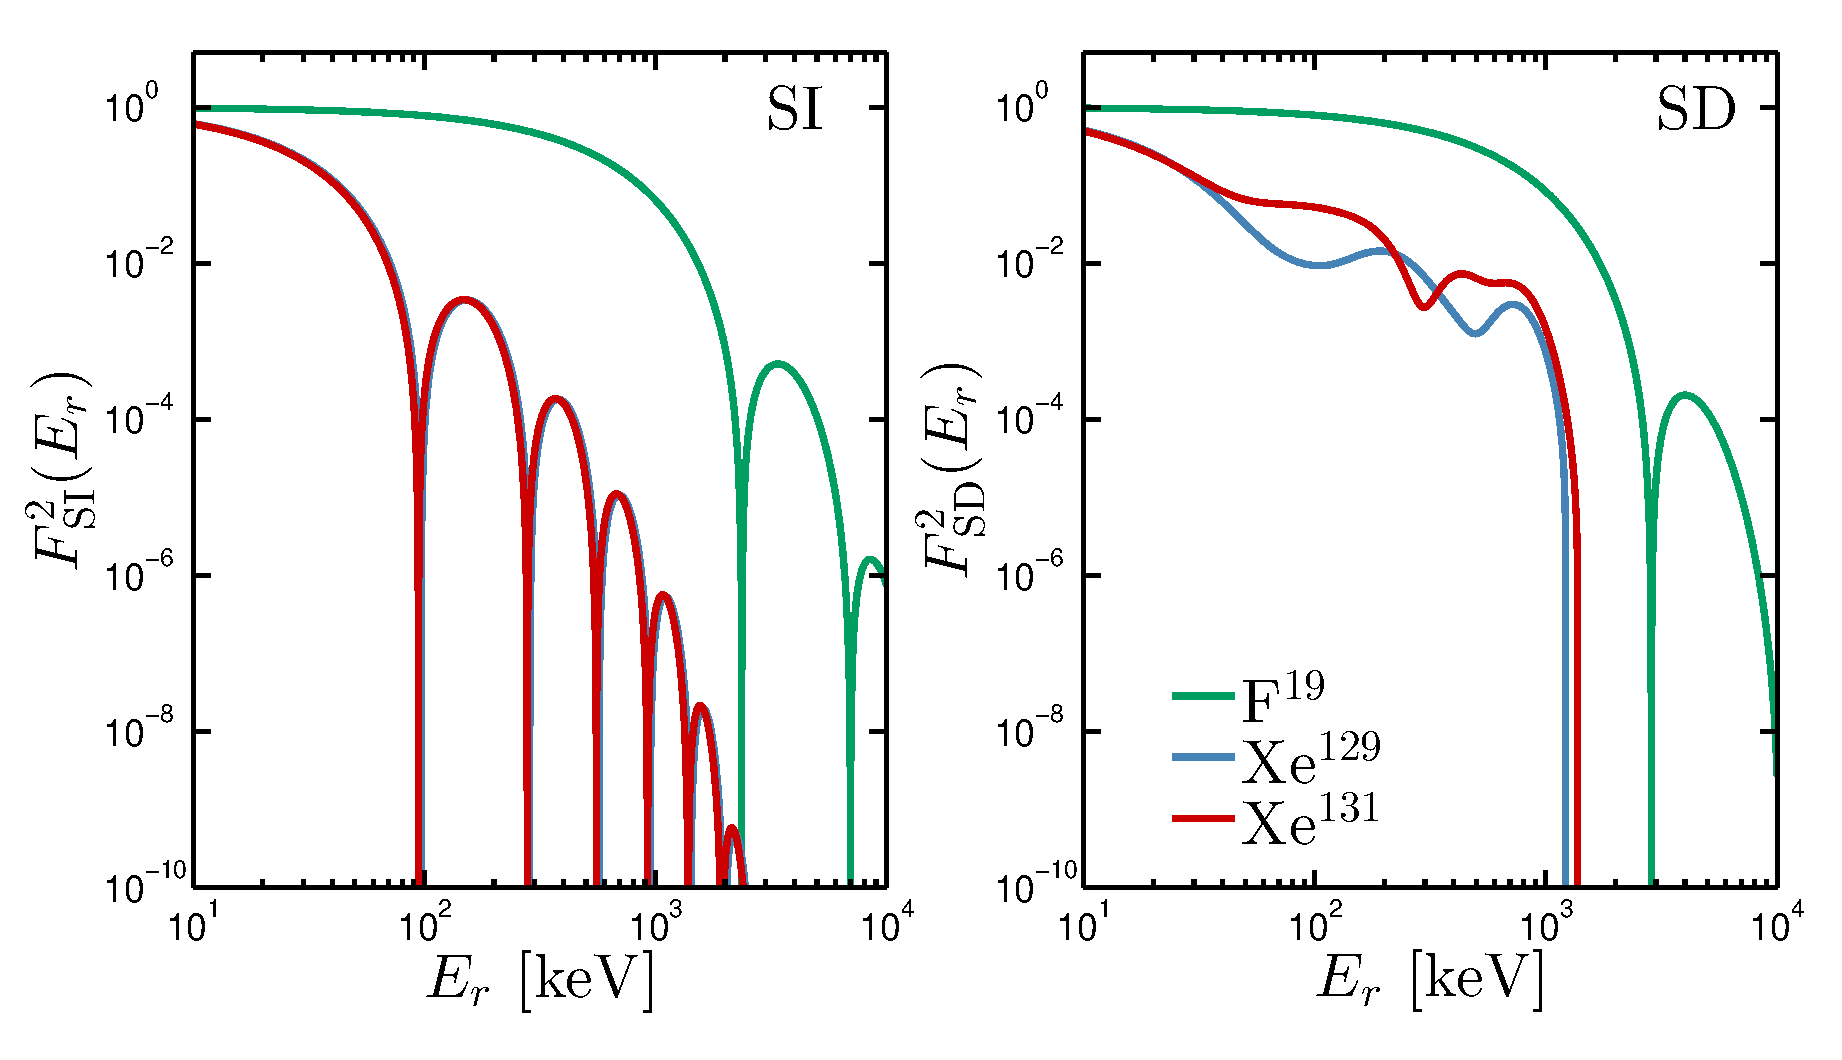
\includegraphics[width=0.97\textwidth]{Figures/FormFactors.eps}
\caption[Fluorine and xenon form factors]{Squared form factors for $^{19}$F (green), $^{129}$Xe (blue) and $^{131}$Xe (red) for spin-independent (left) and spin-dependent (right) interactions.}\label{fig:FormFactors}
\end{center}
\end{figure}

\subsection{Detector effects}
The goal of a direct detection experiment is to measure $\textrm{d}R(t)/\textrm{d}E_r$ in some way. The way this is achieved depends on the technology of the experiment as we will discuss in Sec.~\ref{sec:direct_expts}, however we can first define several key detector effects that modify the observed event rate. One of the most important detector effects to consider is the threshold energy $E_{\rm th}$. Experiments cannot observe arbitrarily small energies, meaning that all analyses will take place using recoils that have been observed above a given threshold. This energy may be a facet of the detector itself in cases where energies must be large enough to yield a detectable signal. The threshold energy is also sometimes enforced during data analysis, for example if there are large backgrounds or background uncertainties at low energies. Because $\textrm{d}R/\textrm{d}E_r$ drops exponentially with energy, achieving low $E_\textrm{th}$ has a big payoff in the total event rate so widening the signal acceptance to lower energies is a central goal of direct detection experiments in general. Lower thresholds are also of course required to access smaller WIMP masses. As well as a lower limit, we will also define a maximum cutoff energy, $E_\textrm{max}$, which is imposed in some experiments to deal with higher energy backgrounds or as the boundary of a signal acceptance region.

Real detectors will not be able to perfectly reconstruct the energy of a recoil. This is normally parameterised in terms of an energy resolution $\sigma(E_r)$ which must be taken into account when predicting the recoil energy spectrum that would be observed in an experiment. Extracting signals from a scattering event may also not be consistently efficient at all energies. This is accounted for in terms of an efficiency function $\epsilon(E_r)$ which typically drops off towards the threshold of the experiment. We define the `detector' recoil spectrum as a modification of the true recoil spectrum in the following way,
\begin{equation}
 \frac{\textrm{d}R_{\rm det}(t)}{\textrm{d}E_r} = \epsilon (E_r) \int_0^\infty K(E_r,E'_r)\frac{\textrm{d}R(t)}{\textrm{d}E'_r} \textrm{d} E'_r
\end{equation}
where $K(E_r,E'_r)$ is a Gaussian smoothing kernel,
\begin{equation}
K(E_r,E'_r) = \frac{1}{\sqrt{2\pi}\sigma(E_r)}e^{-\frac{(E_r-E_r')^2}{2\sigma^2(E_r)}} \, ,
\end{equation}
for an energy dependent resolution $\sigma(E_r)$. Most experiments will have some conversion factors that translate the signals observed in the detector into a recoil energy in keV and accounting for effects like quenching. We neglect these and their corresponding uncertainties as they will be very experiment specific. We also assume that our simulated experiments can achieve perfect discrimination between electron and nuclear recoils, meaning our mock data will consist solely of the latter. 

The total number of events seen in an experiment is controlled by both the physical size of the detector (i.e. its total mass $M$) and the running time $\Delta t = t_f-t_i$. This is usually expressed as an exposure with dimensions of mass-time. Including the aforementioned experimental factors this finally leaves us with a formula for the number of WIMP events to expect in a real experiment,
\begin{equation}
N_\textrm{WIMP} = M \int_{t_i}^{t_f} \int_{E_{\rm th}}^{E_{\rm max}} \frac{\textrm{d}R_{\rm det}(t)}{\textrm{d}E_r} \, \textrm{d}E_r \, \textrm{d}t \, . 
\end{equation}


\section{WIMPs in the Milky Way}\label{sec:direct_MW}
Predictions for signals in direct detection experiments require not only the description of the interaction between the dark matter particle and the target nuclei but also how those particles are phase space distributed in the region of the Milky Way around the Solar System. As introduced in the previous Section the key aspects are the local density, the velocity distribution and the velocity of the Earth through the halo which boosts the distribution into the laboratory frame. Since a dominant component of this thesis is involved with the astrophysics dependence we will now describe each of these in turn and their various sources of uncertainty.

\subsection{Local density}\label{sec:direct_density}
The local density of WIMPs, $\rho_0$, appears in Eq.~(\ref{eq:finaleventrate}) as a multiplicative factor. Since it shares this role with the interaction cross section, we require external knowledge of $\rho_0$ to break the degeneracy as we would not be able to constrain $\sigma$ otherwise. Measurements of the dark matter density are classed as either `local' or `global'. Local measurements are made by estimating the shape of the gravitational potential in the nearby Milky Way. This requires surveys of the vertical motions of nearby stars. There have been many determinations of $\rho_0$ made using this technique in the past dating back to the measurements of Kapteyn \etal~in the 1920s and 30s, see e.g. Refs.~\cite{Salucci:2010qr,Smith:2011fs,Bovy:2012tw,Garbari:2012ff,Zhang:2012rsb,Bovy:2013raa}. Global measurements on the other hand require first building a mass model for the Milky Way halo and then using tracers of the dynamics of the halo, such as the rotation curve, to fit the parameters of the model and subsequently infer the density at the Earth's Galactic radius. Measurements of this kind, e.g. Refs.~\cite{Weber:2009pt,Catena:2009mf,Iocco:2011jz,Nesti:2013uwa,Sofue:2015xpa,Pato:2015dua}, typically have larger systematic uncertainties than local determinations.

Estimates of $\rho_0$ have been historically variable with global measurements generally favouring slightly larger values. Recently however the two methods have started to converge~\cite{Bovy:2013raa,Piffl:2014mfa}.  Recent high precision surveys such as Gaia~\cite{Bailer-Jones:2013saa} will allow future measurements with small statistical uncertainties. However systematic modelling uncertainties will still be the dominant source of error, so methods for extracting the local density that rely on small numbers of assumptions will become essential~\cite{Silverwood:2015hxa}. The canonical value used by experiments is $\rho_0 = 0.3$~GeV~cm$^{-3}$ which we will also use to avoid unnecessary translation issues between our results and experimental limits. In the event of a positive WIMP signal an accurate value for the local density will be important for allowing an unbiased measurement of the cross section to relate to SUSY models, for example. However as many of our results are comparative in nature the precise value is not of huge importance, provided there is consistency. 

\subsection{Laboratory velocity}\label{sec:direct_vlab}
\begin{figure}
	%trim option's parameter order: left bottom right top
	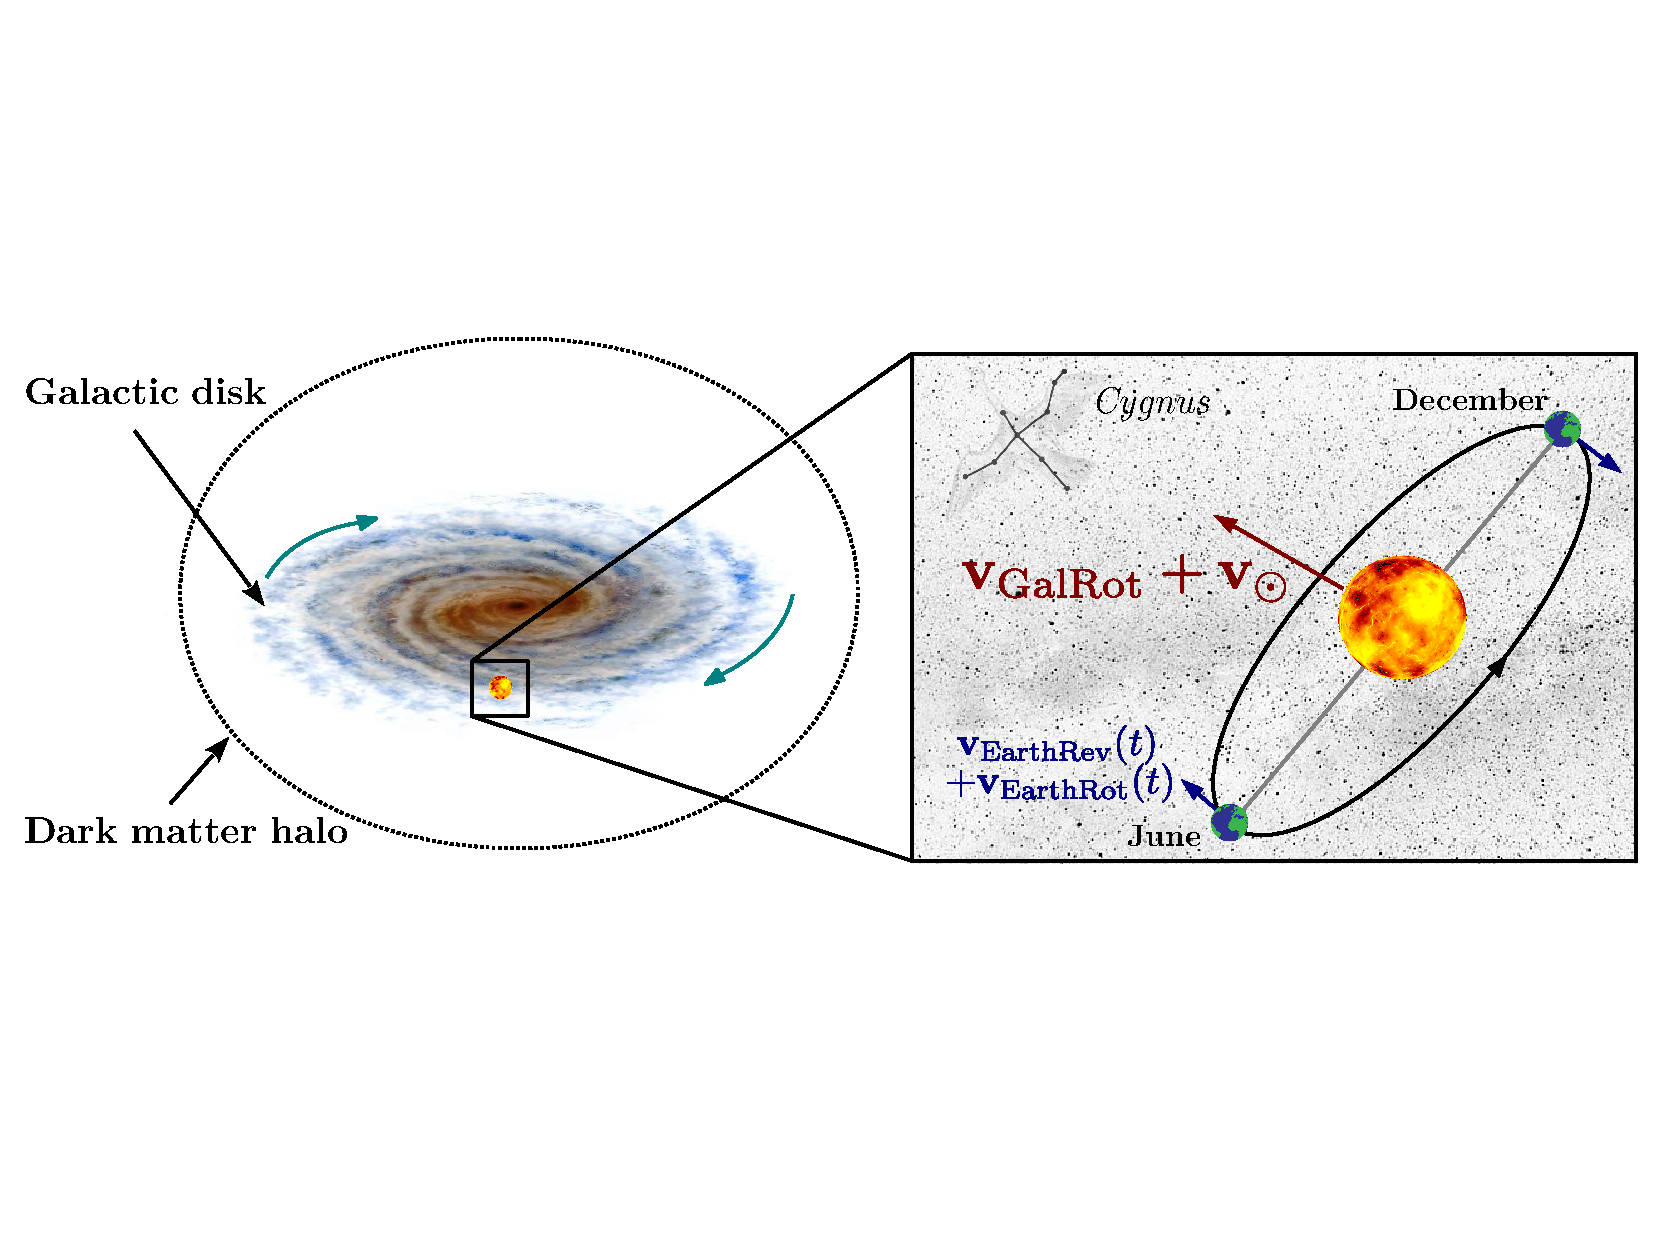
\includegraphics[trim = 0mm 50mm 0mm 50mm, clip, width=\textwidth]{Figures/labvelocity.pdf}
	\caption[Diagram of the components of the lab velocity]{Diagram of the components of the lab velocity.}
	\label{fig:labvelocity}
\end{figure}
The velocity distribution of WIMPs in the rest frame of the laboratory is obtained through a Galilean transformation of the Galactic frame distribution by the time dependent laboratory velocity ${\bf v}_{\rm lab}(t)$. This boost into the lab frame is responsible for time dependence, and for an isotropic Galactic frame distribution, is the sole source of the anisotropy in recoil directions (to be explored in Chapter~\ref{chapter:directional}). The lab velocity is,
\begin{equation}
\textbf{v}_\textrm{lab}(t) = {\bf v}_{\rm GalRot} + {\bf v}_\odot + {\bf v}_{\rm EarthRev}(t) + {\bf v}_{\rm EarthRot}(t) \, ,
\end{equation}
which is the sum of the bulk rotation of the local standard of rest (LSR) around the Galactic center, ${\bf v}_{\rm GalRot}$, the peculiar velocity of the Solar System with respect to the LSR, ${\bf v}_\odot$, the Earth's revolution around the sun, ${\bf v}_{\rm EarthRev}$, and the Earth's rotation, ${\bf v}_{\rm EarthRot}$.

When working in the laboratory frame we can use a North-West-Zenith coordinate system to describe each of these velocties. The astrophysical literature however will most often quote values in the Galactic coordinate system, ($U$,$V$,$W$), which point towards the Galactic center, the direction of Galactic rotation and the Galactic north pole respectively. We will also occasionally make use of Galactic longitude and latitude $(l,b)$ which are defined for a velocity $v$,
\begin{equation}
 \textbf{v} = v \, \begin{pmatrix} \cos l \cos b \\ \sin l \cos b \\ \sin b \end{pmatrix} \, .
\end{equation}

The dominant contribution to the lab velocity is ${\bf v}_{\rm GalRot}$. The velocity of the LSR is set up in Galactic coordinates as (0, $v_0$, 0) where $v_0$ is the circular rotation speed of the Milky Way. The value of $v_0$ is also the dominant source of uncertainty in $\textbf{v}_\textrm{lab}$. The standard value currently in use is $v_0\sim220$~km~s$^{-1}$~\cite{Kerr:1986hz}. The rotation of the Milky Way has been measured in various ways. For instance, measurements of the proper motions of nearby stars and Sgr A* located at the Galactic center can be used to constrain the quantity $(v_0+V_\odot)/R_\odot$ where $V_\odot$ is the second component of $\textbf{v}_\odot$ and $R_\odot$ is the Solar Galactic radius. Given independent constraints on the Solar peculiar velocity and radius one can combine measurements to arrive at a constraint on $v_0$. However, as noted by Lavalle \& Magni~\cite{Lavalle:2014rsa} because these estimates depend upon the prior assumptions made about other parameters, combining measurements of, for instance $R_\odot$ and $V_\odot$ from different sources may lead to spurious resulting values and underestimated errors. A study by McMillan \& Binney~\cite{McMillan:2009yr} for example found that values of the speed of the local standard of rest are heavily dependent on the model used for the rotation curve, quoting values of $v_0$ from $200 \pm 20$~km~s$^{-1}$ to $279 \pm 33$~km~s$^{-1}$. The peculiar velocity on the other hand is believed to possess a reasonably small uncertainty. A value commonly used from Schoenrich \etal~\cite{Schoenrich:2009bx} gives $\textbf{v}_\odot = (11.1,12.24,7.25)$~km~s$^{-1}$ in Galactic coordinates with roughly 1~km~s$^{-1}$ sized systematic errors. 

As shown in Fig.~\ref{fig:labvelocity} the velocities ${\bf v}_{\rm EarthRev}$ and ${\bf v}_{\rm EarthRot}$ are, respectively, responsible for the annual and diurnal~\cite{Bozorgnia:2011tk} modulation effects. For us they are known with effectively perfect precision. The calculation of these two components of the lab velocity and the necessary transformations between the Galactic and laboratory coordinate systems are presented in Appendix~\ref{app:labvelocity}. We display the time dependence induced in the total integrated event rate, $R$, due to these velocities in Fig.~\ref{fig:AnnualDailyModulation}. As can be seen, the phase and amplitude of the diurnal modulation is dependent on the location of the experiment.

\begin{figure}
\begin{center}
\includegraphics[width=0.95\textwidth]{Figures/AnnualDailyModulation.eps}
\caption[Annual and daily modulation signal]{Annual and daily modulation signal for three WIMP masses 50, 100 and 150 GeV (from top to bottom). The closeup shows the daily modulation signal for a 50 GeV WIMP for xenon target experiments located at three different locations. The event rate is calculated by integrating $\textrm{d}R(t)/\textrm{d}E_r$ over $E_r$ above a threshold which we set to 5 keV. The cross section in each case is $\sigma_p^{\rm SI} = 10^{-45}$~cm$^2$.}\label{fig:AnnualDailyModulation}
\end{center}
\end{figure}

\subsection{Velocity distribution}\label{sec:direct_fv}
The scattering rate is dependent on the Earth frame DM velocity distribution in the form of its mean inverse speed $g(\vmin,t)$. The true form of the local velocity distribution is unknown. However, unlike the lab velocity and local density, it cannot be measured astronomically. In principle only direct detection experiments have access to it. Hence we must pick a form for the distribution corresponding to a model for the Milky Way dark matter halo. If the density profile is analytic then the velocity distribution can be found by solving the Jeans equation. Alternatively a form can be extracted from the results of N-body or hydrodynamic simulations of Milky Way-like halos. As with the local density, the choice of $f(\textbf{v})$ will affect the predictions for the event rate. However the velocity distribution affects not just the total event rate but also the recoil energy dependence. This is an important but subtle point and can be exploited to give rise to considerable uncertainty in WIMP exclusion limits.

Most direct detection analyses are performed under a simple assumption for the Milky Way halo known as the standard halo model (SHM)~\cite{Green:2011bv}. This is a spherically symmetric isothermal halo model. Its $1/r^2$ density profile yields a Maxwell-Boltzmann (MB) velocity distribution with peak speed $v_0 = 220 \kms$ and dispersion\footnote{The relationship between the dispersion and circular speed is a consequence of a $1/r^2$ density profile, so relaxing this assumption means that $v_0$ and $\sigma_v$ are no longer connected.} $\sigma_v = v_0/\sqrt{2} \approx 156 \kms$. The distribution is most often truncated at the escape speed of the galaxy. The measurement from the radial velocity of RAVE stars is: $\vesc = 533^{+54}_{-41} \kms$~\cite{Piffl:2013mla}. The velocity distribution in the laboratory frame is therefore given by:
\begin{equation}\label{eq:shm}
f_\mathrm{SHM}(\mathbf{v},t) = \frac{1}{(2\pi \sigma_v^2)^{3/2}N_\mathrm{esc}} \, \exp \left( - \frac{|\mathbf{v} - \mathbf{v}_\textrm{lab}(t)|^2}{2\sigma_v^2}\right) \, \Theta (\vesc - |\mathbf{v} - \mathbf{v}_\textrm{lab}(t)|)\,, 
\end{equation}
with the normalisation constant,
\begin{equation}
N_\mathrm{esc} = \erf \left( \frac{\vesc}{\sqrt{2}\sigma_v}\right) - \sqrt{\frac{2}{\pi}} \frac{\vesc}{\sigma_v} \exp \left( -\frac{\vesc^2}{2\sigma_v^2}   \right)\,.
\end{equation}
Evaluating Eq.~(\ref{eq:gvmin}) for this velocity distribution gives for the mean inverse speed,
\begin{equation}\label{eq:gvmin_SHM}
g(\vmin,t) =
\begin{cases}
\frac{1}{v_\textrm{lab}(t)} & z<y\, , x<|y-z| \\
\frac{1}{2 N_{\rm esc} v_\textrm{lab}(t)} \left( \erf{(x+y)} - \erf{(x-y)} - \frac{4y}{\sqrt{\pi}} e^{-z^2}\right) & z>y \, , \, x<|y-z| \\
\frac{1}{2 N_{\rm esc} v_\textrm{lab}(t)} \left( \erf{(z)} - \erf{(x-y)} - \frac{2(y+z-x) }{\sqrt{\pi}} e^{-z^2}\right) & |y-z| < x<y+z \\
0 & y+z< x
\end{cases}
\end{equation}
where $x = \vmin/\sqrt{2}\sigma_v$, $y \equiv y(t) = v_{\rm lab}(t)/\sqrt{2}\sigma_v$ and $z = \vesc/\sqrt{2}\sigma_v$.

In order to maintain consistency when comparing experimental results it is important to establish some baseline halo model. The lack of a better motivated alternative and its simplicity mean the SHM can fill this role. Interestingly however, a number of recent hydrodynamic simulations suggest that a simple MB distribution may in fact be sufficient to describe the local velocity distribution \cite{Bozorgnia:2016ogo,Kelso:2016qqj,Sloane:2016kyi}. However many other hydrodynamic simulations, as well as earlier N-body simulations, presented persistent evidence for non-Maxwellian structure in Milky Way-like halos~\cite{Lisanti:2010qx,Kuhlen:2012ft,Fornasa:2013iaa,Butsky:2015pya}. The matter has not yet been conclusively settled and, critically for direct detection experiments, there is the possibility that the dark matter distribution at the Earth's Galactic radius could contain significant departures from the smooth isotropic properties of the SHM~\cite{Vogelsberger:2008qb,Maciejewski:2010gz,Mao:2012hf}. The velocity distribution may also contain additional features and substructures such as debris flows~\cite{Lisanti:2011as,Kuhlen:2012fz}, tidal streams~\cite{Freese:2003tt,Purcell:2012sh}, a co-rotating dark disk~\cite{Read:2009iv,Kuhlen:2013tra,Schaller:2016uot} or a `shadow bar'~\cite{Petersen:2016xtd,Petersen:2016vck}.

We consider two classes of substructure in this work which are motivated by results from N-body simulations, but also importantly have contrasting velocity structures so that they can be compared under a range of scenarios.

\textbf{Streams}: The local velocity distribution may contain substructure due to the tidal disruption and stripping of satellite galaxies or dark subhalos of the Milky Way. The slow accretion of material gives rise to a streams of dark matter particles wrapping the Galaxy some of which may intersect the stellar disk. Streams are seen generically in simulations of Milky Way-like galaxies as smaller subhalos become absorbed by their larger host and are in fact an inevitable consequence of the hierarchical growth of structure. There is also motivation for the existence of streams close to the Solar System. There have been observations in the past of collective linear motions of stars with narrow velocity dispersion consistent with a tail of stripped material from the nearby Sagittarius dwarf galaxy~\cite{Newberg:2003cu,Yanny:2003zu,Majewski:2003ux,Luque:2016nsz}. Furthermore simulations of the Sagittarius dwarf galaxy have found that the dark matter component of the stream could be significantly more extended than the stellar component and could hence give a sizable population of stream dark matter in direct detection experiments~\cite{Purcell:2012sh}.

If such a stream passed through the Solar System it would exist as a separate component of the local dark matter distribution with speeds tightly concentrated around a single velocity which would not necessarily be aligned with $\textbf{v}_\textrm{lab}$. We construct a model that assumes a fixed fraction of the local density is contained in the form of a tidal stream, described by Galactic frame velocity $\mathbf{v}_\textrm{str}$ and dispersion $\sigma_\mathrm{str}$. The velocity distribution of the stream is given by,
\begin{equation}
f_\mathrm{Str}(\mathbf{v},t) = \frac{1}{(2\pi \sigma_\textrm{str}^2)^{3/2}} \, \exp \left( - \frac{(\mathbf{v} - (\mathbf{v}_\textrm{lab}(t)+\mathbf{v}_\textrm{str}))^2}{2\sigma_\textrm{str}^2}\right) \,,
\end{equation}
and the full velocity distribution of the ``SHM+Str'' model is given by,
\begin{equation}
 f_\mathrm{SHM+Str}(\mathbf{v}) = \left(1-\frac{\rho_\mathrm{str}}{\rho_0}\right)f_\mathrm{SHM}(\mathbf{v},t) + \frac{\rho_\mathrm{str}}{\rho_0} f_\mathrm{Str}(\mathbf{v},t) \, .
\end{equation}
where $\rho_0$ is the SHM density and $\rho_\mathrm{str}$ is the stream density. The mean inverse speed for the stream has the same formula as for the SHM, Eq.~(\ref{eq:gvmin_SHM}) with $y~=~|\textbf{v}_\textrm{lab}(t)~+~\textbf{v}_\textrm{str}|/v_0$. Due to the spatially and kinematically localised nature of these features they give rise to prominent directional signatures in the recoil spectrum~\cite{Lee:2012pf,O'Hare:2014oxa}, as well as adding non-sinusoidal modifications to the annual modulation signals~\cite{Savage:2006qr}. 


\textbf{Debris flow}: Debris flows are another form of substructure that have appeared in N-body simulations such as Via Lactea II~\cite{Kuhlen:2008qj,Kuhlen:2012fz}. Like streams these are kinematically localised, characterised by a speed $v_f$, though unlike streams they are spatially extended features which form from the incomplete phase mixing of material during the formation of the halo. Following Ref.~\cite{Kuhlen:2012fz} we assume a model for the debris flow in which the velocity distribution is isotropic in the Galactic frame and a delta function in speed centered on $v_f$,
\begin{equation}
 f_\mathrm{DF}(\mathbf{v},t) = \frac{1}{4\pi v_f^2} \,\delta(|\mathbf{v}-\mathbf{v}_\textrm{lab}|-v_f) \, .
\end{equation}
So the distribution of a DF (in the laboratory frame) is a shell of radius $v_f$ centered on $\textbf{v}_\textrm{lab}$. Now, as with the SHM+Str model we combine the debris flow with the SHM as a fixed fraction of the local density:
\begin{equation}
 f_\mathrm{SHM+DF}(\mathbf{v},t) = \left(1-\frac{\rho_f}{\rho_0}\right)f_\mathrm{SHM}(\mathbf{v},t) + \frac{\rho_f}{\rho_0} f_\mathrm{DF}(\mathbf{v},t) \, .
\end{equation}
The mean inverse speed for this model is,
\begin{equation}
g(\vmin,t) =
\begin{cases}
\frac{1}{v_f} & \vmin < v_f-v_{\rm lab}(t) \\
\frac{v_f+v_{\rm lab}(t) - \vmin}{2v_f v_{\rm lab}(t)} & v_f-v_{\rm lab}(t)<\vmin <v_f+v_{\rm lab}(t) \\
0 & \vmin <v_f+v_{\rm lab}(t) \\
\end{cases}
\end{equation}

These benchmark velocity distributions along with the SHM are shown in Fig.~\ref{fig:polar}, while a summary of the benchmark parameter values used for each halo model is given in Table~\ref{tab:astrobenchmarks}. For the stream we use an estimate of the velocity of the Sagittarius stream from Ref.~\cite{Savage:2006qr}. However we assume that it comprises a significantly larger fraction of the local density than suggested by simulations, typically around the 1\% level~\cite{Vogelsberger:2008qb,Maciejewski:2010gz}. This allows us to make a clear distinction between our benchmark models. For the debris flow we use the parameters derived in the semi-analytic model of Ref.~\cite{Kuhlen:2012fz} based on the Via Lactea II simulation~\cite{Kuhlen:2008qj}. Although the debris flow in this simulation exhibited some velocity dispersion as well as a small bias towards directions tangential to the Galactic rotation, the simple isotropic model was found to capture the main features of the recoil spectrum.

Beside the benchmark velocity distributions in Fig.~\ref{fig:polar} we show sets of recoil energy spectra for a range of WIMP masses. For each benchmark model we see the same basic shape due to the SHM: an exponentially decreasing event rate which is cut off above some maximum energy set by the escape velocity. When streams and debris flows are included they induce an enhancement in the event rate for energies below a certain value which is set by the stream velocity or flow velocity respectively. 


\begin{table}[t]\centering
\ra{1.3}
\begin{tabularx}{\textwidth}{l|lll}
\hline\hline
\multirow{2}{*}{\bf Lab velocity}& Galactic rotation & $\textbf{v}_\textrm{GalRot}$ & (0, $v_0$, 0) km s$^{-1}$ \\
				 & Peculiar velocity & $\textbf{v}_\odot$ & (11.1, 12.24, 7.25) km s$^{-1}$ \\
\hline
\multirow{4}{*}{\bf SHM} & Local density & $\rho_0$ 		& $0.3 \, \mathrm{GeV} \, \mathrm{cm}^{-3}$\\
				& Circular speed & $v_0$ 	& $220 \kms$\\
				& Velocity dispersion& $\sigma_v$ 		& $156 \kms$\\
				& Escape speed& $\vesc$ & $533 \kms$\\
\hline
\multirow{3}{*}{{\bf Stream}}& Velocity & $\sigma_\textrm{str}$ 		& $10 \, \kms$\\
				& Dispersion& $\textbf{v}_\textrm{str}$ 	& $400\times(0,0.233,-0.970) \kms$\\
				& Density & $\rho_\textrm{str}/\rho_0$ 		& $0.1$\\
\hline
\multirow{2}{*}{{\bf Debris flow}} & Flow speed & $v_f$ 		& $340 \, \kms$\\
				& Density & $\rho_f/\rho_0$ 		& $0.22$\\
\hline\hline
\end{tabularx}
\caption[Astrophysical benchmark parameters]{Astrophysical benchmark parameters for the time independent components of the lab velocity, the standard halo model alone, stream and debris flow. In all examples, unless otherwise specified, the above parameters are used.}
\label{tab:astrobenchmarks}
\end{table}


\begin{figure}
\begin{center}
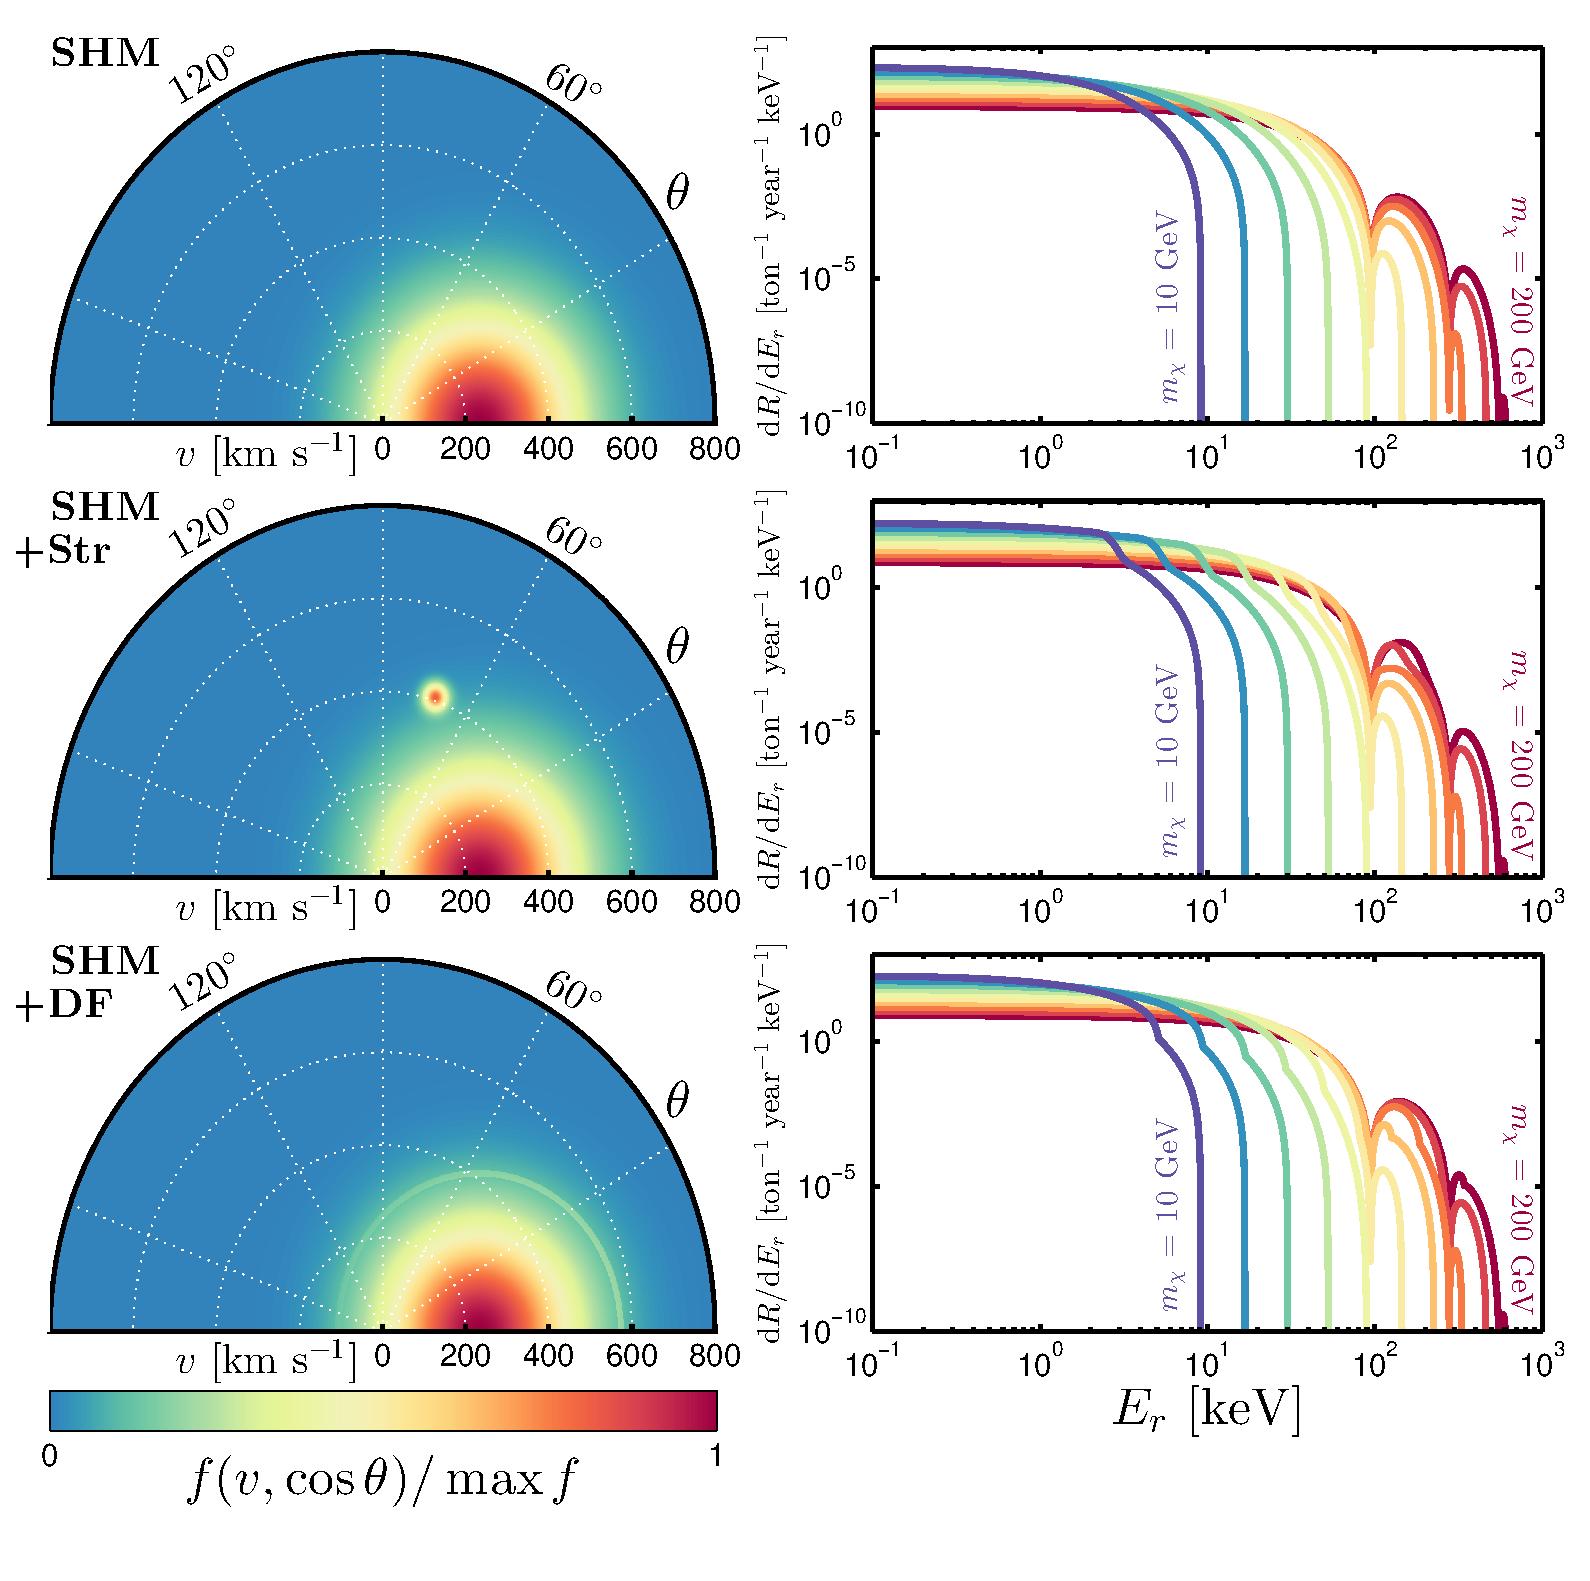
\includegraphics[width=0.97\textwidth]{Figures/fvEventRates.eps}\\
\caption[Benchmark velocity distributions and corresponding event rates]{ {\bf Left}: benchmark velocity distributions. We plot the velocity distribution for the SHM (top), SHM + Str (middle) and SHM + DF (bottom). The polar angle $\theta$ is measured with respect to $\mathbf{v}_\textrm{lab}$ and we have integrated $2\pi$ over the remaining azimuthal angle. {\bf Right:} corresponding SI xenon event rate energy spectra for each halo model over a range of logarithmically spaced masses between $m_\chi = 50$ to 200~GeV (blue to red).}\label{fig:polar}
\end{center}
\end{figure}
% shm should be 2pi larger than stream

Describing the velocity distribution is an important consideration for excluding or detecting dark matter in direct detection experiments. A failure to properly account for uncertainties in the DM velocity distribution may lead to biased measurements of the WIMP mass and cross section with a future signal~\cite{Peter:2011eu}. It will therefore be imperative to include these uncertainties in fits to direct detection data. This can be done by fitting to phenomenological models for the local distribution~\cite{Billard:2010jh,Lee:2012pf,O'Hare:2014oxa}, or by attempting to integrate out the astrophysics dependence of the DM signal so that comparisons can be made between exclusion limits from different experiments in a `halo-independent' way~\cite{Fox:2010bz,Fox:2010bu,Frandsen:2011gi,Gondolo:2012rs,DelNobile:2013cta,Fox:2014kua,Feldstein:2014gza,Anderson:2015xaa,Gelmini:2016pei,Kahlhoefer:2016eds,Ibarra:2017mzt}. Alternatively one can use empirical parameterisations of the speed distribution to account for astrophysical uncertainties, although this may lead to weakened constraints on other DM parameters~\cite{Peter:2011eu,Kavanagh:2013wba,Kavanagh:2013eya}. In the next Chapter we will explore model dependent and independent approaches for dealing with substructure in the velocity distribution with directional detectors.

\section{Experiments}\label{sec:direct_expts}
A direct detection experiment essentially consists of a fixed collection of particles called the `target' that are carefully monitored for the emission of certain signals (such as photons, charge or heat) which can be attributed to scattering events between the target and other particles. These particles can either be dark matter, or a background, which is anything else. In the event of an excess in the number of recoil events detected in the experiment over the expectation, then the measured $\textrm{d}R(t)/\textrm{d}E_r$ of those events can in principle be used to extract the properties of the WIMP. In the scenario that no unexplained excesses are detected then ranges of parameter values can be excluded. Real experiments are fraught with a range of complications related to backgrounds that we will now summarise. We also discuss some of the specific technological designs of certain current experiments and summarise the existing constraints.

\subsection{Backgrounds}
Dark matter scattering interactions are rare. Hence the most important factor for experiments to consider are backgrounds. To identify a signal which may produce less than $10^{-5}$ events per kg-day, ultra-low background conditions are needed. Backgrounds can be reduced at a number of stages. The first stage is to shield the detector volume as much as possible. Operating a detector deep underground or inside a mountain with a considerable distance of ground between the sky and the experiment can typically reduce the cosmic ray flux exponentially with (water equivalent) depth~\cite{Mei:2005gm}. Cosmic rays, in particular muons, must be shielded since they produce showers of up to GeV-scale neutrons in spallation reactions with the surroundings~\cite{Mei:2005gm}. Of all types of background particle, neutrons are the most problematic as their nuclear recoil signal, if they reach the detector, is almost identical to dark matter. 

In addition to cosmic backgrounds, both the environment and the experimental apparatus will be contaminated with radioactive isotopes. Radiogenically produced neutrons as well as Compton scattering and electron pair production due to $\gamma$ radiation are the most significant radioactive backgrounds. These require a second stage of background shielding surrounding the detector volume with additional layers of material such as lead or water tanks to veto environmental radiation. Water tanks can be used as `active' vetos which allow an experiment to reject events in the detector that are coincident with events in the water. Radioactive decays that are produced in the apparatus close to the detector, for example in the shielding itself, also need to be reduced as much as possible by carefully selecting especially radiopure materials. Decays produced due to impurities in the target material itself cannot be shielded so must be reduced as much as possible during manufacture. In detectors using crystalline materials such as CDMS, CRESST and CoGeNT, radioactive contaminants with large ionic radii such as radium, uranium and thorium are mostly rejected in the crystal growing process as they do not fit within the lattice spacing~\cite{Munster:2014mga}. Experiments using noble gases also have to contend with naturally occurring radioactive isotopes. Argon for example has a cosmogenically activated isotope ($^{39}$Ar) so experiments such as DarkSide find sources from deep underground~\cite{Back:2012pg}. In xenon the naturally occurring radioactive isotopes have half lives either short enough or long enough to not affect the experiment, but contamination from krypton and radon isotopes have led the XENON100, XMASS and LUX collaborations to develop special techniques to detect and extract quantities occurring at less than a part per quadrillion~\cite{Lindemann:2013kna}.

Whatever backgrounds that remain must be rejected at the level of the experimental design and analysis. The approach that has proven particularly powerful in certain experiments is electronic/nuclear recoil discrimination. WIMPs are much more likely to induce a nuclear recoil signal than an electron recoil signal meaning an experiment that can discriminate between the two can achieve a much greater level of sensitivity. Distinguishing between different sources of background is more efficient if an experiment can measure multiple types of signal from an event, e.g. scintillation photons, ionisation or phonons. WIMPs are also very unlikely to induce multiple scattering events compared with backgrounds. Linking series of recoil by either locating them in the detector volume or with time-tagging can be another useful approach for eliminating likely backgrounds. Additionally in experiments in which recoil sites are located, the outer layers of the detector volume itself can be used as a self-veto, with only the inner portion comprising the `fiducial' detector volume used for analysis. Ultimately though it is impossible to completely eliminate backgrounds so the final stages involve reducing backgrounds at the level of the analysis. This involves the modelling of backgrounds, use of detector calibration data, and defining signal regions in which the observed backgrounds are low. 

The final, though as yet unobserved, background to direct detection experiments are neutrinos from the Sun, the atmosphere as well as a cumulative emission from supernovae called the diffuse supernova background (DSNB). These cannot be shielded or rejected by any other means and dealing with them in standard direct detection experiments requires very high statistics~\cite{Billard:2013qya}. When direct detection experiments reach sizes large enough to observe a background due to coherent neutrino-nucleus scattering the large uncertainty on the expected neutrino flux compared with the low statistics expected from dark matter will limit discovery of certain masses where the two spectra overlap. We discuss the neutrino floor and approaches to deal with it in Chapter~\ref{chapter:nufloor}. 


\subsection{Current experiments}\label{sec:direct_current}
Direct detection experiments can be categorised based on the principle types of signal used to detect scattering events. All current experiments exploit at least one of three possible signals. These are: ionisation charge from liberated electrons/ions; scintillation photons from the excitation and de-excitation of electrons or nuclei in the target atoms; and phonons which are quantised vibrations such as heat or sound waves that propagate through solids. Many of the more recent experiments use a combination of two of these three detection channels. We now describe different broad categories of experimental design based on the state of the target material: noble gases, solid state and superheated fluids\footnote{We also discuss directional detectors in the next Chapter.}.

{\bf Noble gases}: Currently the most sensitive limits on SI cross sections for $m_\chi>20$ GeV are made by the dual phase xenon experiments, Xenon100~\cite{Aprile:2012nq}, LUX~\cite{Akerib:2016vxi}, and PandaX~\cite{Tan:2016zwf}. These experiments operate as time projection chambers (TPCs) in a design originally pioneered by ZEPLIN~\cite{Akimov:2006qw} and Xenon10~\cite{Aprile:2010bt} (the predecessor to Xenon100). The main detector volume is filled with liquid xenon with a smaller volume of gaseous xenon placed at the top of the main tank which collects ionised electrons drifted by an applied electric field. Photomultiplier tubes are arranged to detect both the photons produced as the drifted charge meets the gas phase xenon, as well as the prompt scintillation photons emitted from the initial scattering event. The yields from these different signals is dependent on the type of particle scattering so dual phase xenon TPCs can achieve excellent electronic/nuclear discrimination. Additionally the timing of the signals can be used to locate the event site inside the detector allowing a central fiducial volume to be selected for analysis that is self-shielded from backgrounds. The DarkSide~\cite{Agnes:2015ftt} experiment relies on the same technique but instead with an argon target. Alternatively noble gas experiments can operate solely in the liquid phase: with xenon again in the case of XMASS~\cite{Abe:2013tc} and argon for experiments such as DEAP~\cite{Boulay:2012hq} and MiniCLEAN~\cite{Rielage:2014pfm}. Single phase noble detectors only exploit the scintillation signal but resolve the timing of the received photons to give a `pulse shape' for each event. The advantage of argon in particular in this case is that the duration over which scintillation photons are produced for electronic and nuclear recoils are 6~ns and 1.6~$\mu$s~\cite{Boulay:2006mb} allowing excellent pulse shape discrimination.

{\bf Solid state}: There are two types of solid state detector: cryogenic experiments and crystal scintillators. Cryogenic bolometers such as SuperCDMS~\cite{Agnese:2014aze} and EDELWEISS~\cite{Hehn:2016nll} consist of a germanium target crystal cooled to mK temperatures combined with specialised detectors to measure liberated charge as well as phonons propagating through the solid after a scattering event. The advantage of these experiments are their extremely low energy thresholds. The dedicated single crystal experiment performed by SuperCDMS known as CDMSLite was selected to achieve a particularly low threshold of 0.8 keV (nuclear recoil energy) and currently sets the strongest limits around $m_\chi \sim 3$~GeV~\cite{Agnese:2015nto}. CoGeNT is also a cryogenic germanium experiment but measures only an ionisation signal and searches for an annual modulation to distinguish the signal from the background~\cite{Aalseth:2014eft}. CRESST on the other hand uses CaWO$_4$ crystals and exploits a combination of phonon and scintillation signals to achieve electronic/nuclear recoil discrimination with a 0.3 keV threshold; CRESST-II currently sets the strongest limits below 2 GeV~\cite{Angloher:2015ewa}. The other category of solid state detectors are crystal scintillators which are not operated cryogenically, instead designed to observe photons from molecules in the lattice excited by a scattering event. Scintillators such as DAMA/LIBRA~\cite{Bernabei:2008yh} and KIMS~\cite{Kim:2012rza} consist of collections of ultrapure crystals of NaI or CsI doped with thallium to improve the light emission and transparency of the material. Crystal scintillators have no signal discrimination capabilities so, like CoGeNT, search for an annual modulation in the event rate. DAMA report a 9.6$\sigma$ annual modulation signal with a phase consistent with a dark matter interpretation~\cite{Bernabei:2013xsa}. However the best fit cross sections and masses are ruled out by numerous other experiments\footnote{Arguments involving particle physics~\cite{DelNobile:2015lxa,Chang:2008gd}, astrophysical uncertainties~\cite{Belli:1999nz}, signal channelling~\cite{Savage:2008er} and many others have all been invoked to try and reconcile the tension between DAMA and other experiments.}. The issue has not yet been resolved. Results from experiments also using thallium doped NaI crystals: SABRE~\cite{Shields:2015wka}, Anais~\cite{Amare:2014jta} and DM-Ice~\cite{Cherwinka:2014xta}, will shed light on possible explanations for the signal.

{\bf Superheated fluids}: For spin-dependent (proton) interactions, experiments using superheated droplets of certain liquids: PICO~\cite{Amole:2015lsj,Amole:2015pla}, COUPP~\cite{Behnke:2012ys,Behnke:2008zza}, SIMPLE~\cite{Felizardo:2010mi} and PICASSO~\cite{Archambault:2012pm}, are currently most sensitive among direct detection searches. Superheated liquids are kept at temperatures just below their boiling point, if an event deposits enough energy inside a small enough volume then bubbles are nucleated and can be detected and located by a camera. The advantage of superheated fluids is that the ionising backgrounds from $\gamma$-rays and electrons cannot deposit a high enough energy density to be registered.  The liquids used in these experiments, CF$_3$I, C$_3$F$_8$ C$_2$ClF$_5$ and C$_4$F$_{10}$ all contain $^{19}$F which possesses a large $\langle S_p \rangle$. This has allowed superheated fluid experiments to set some of the strongest constraints on $\sigma_p^{\rm SD}$. 

% need to add new limit from PICO

\begin{figure}
\begin{center}
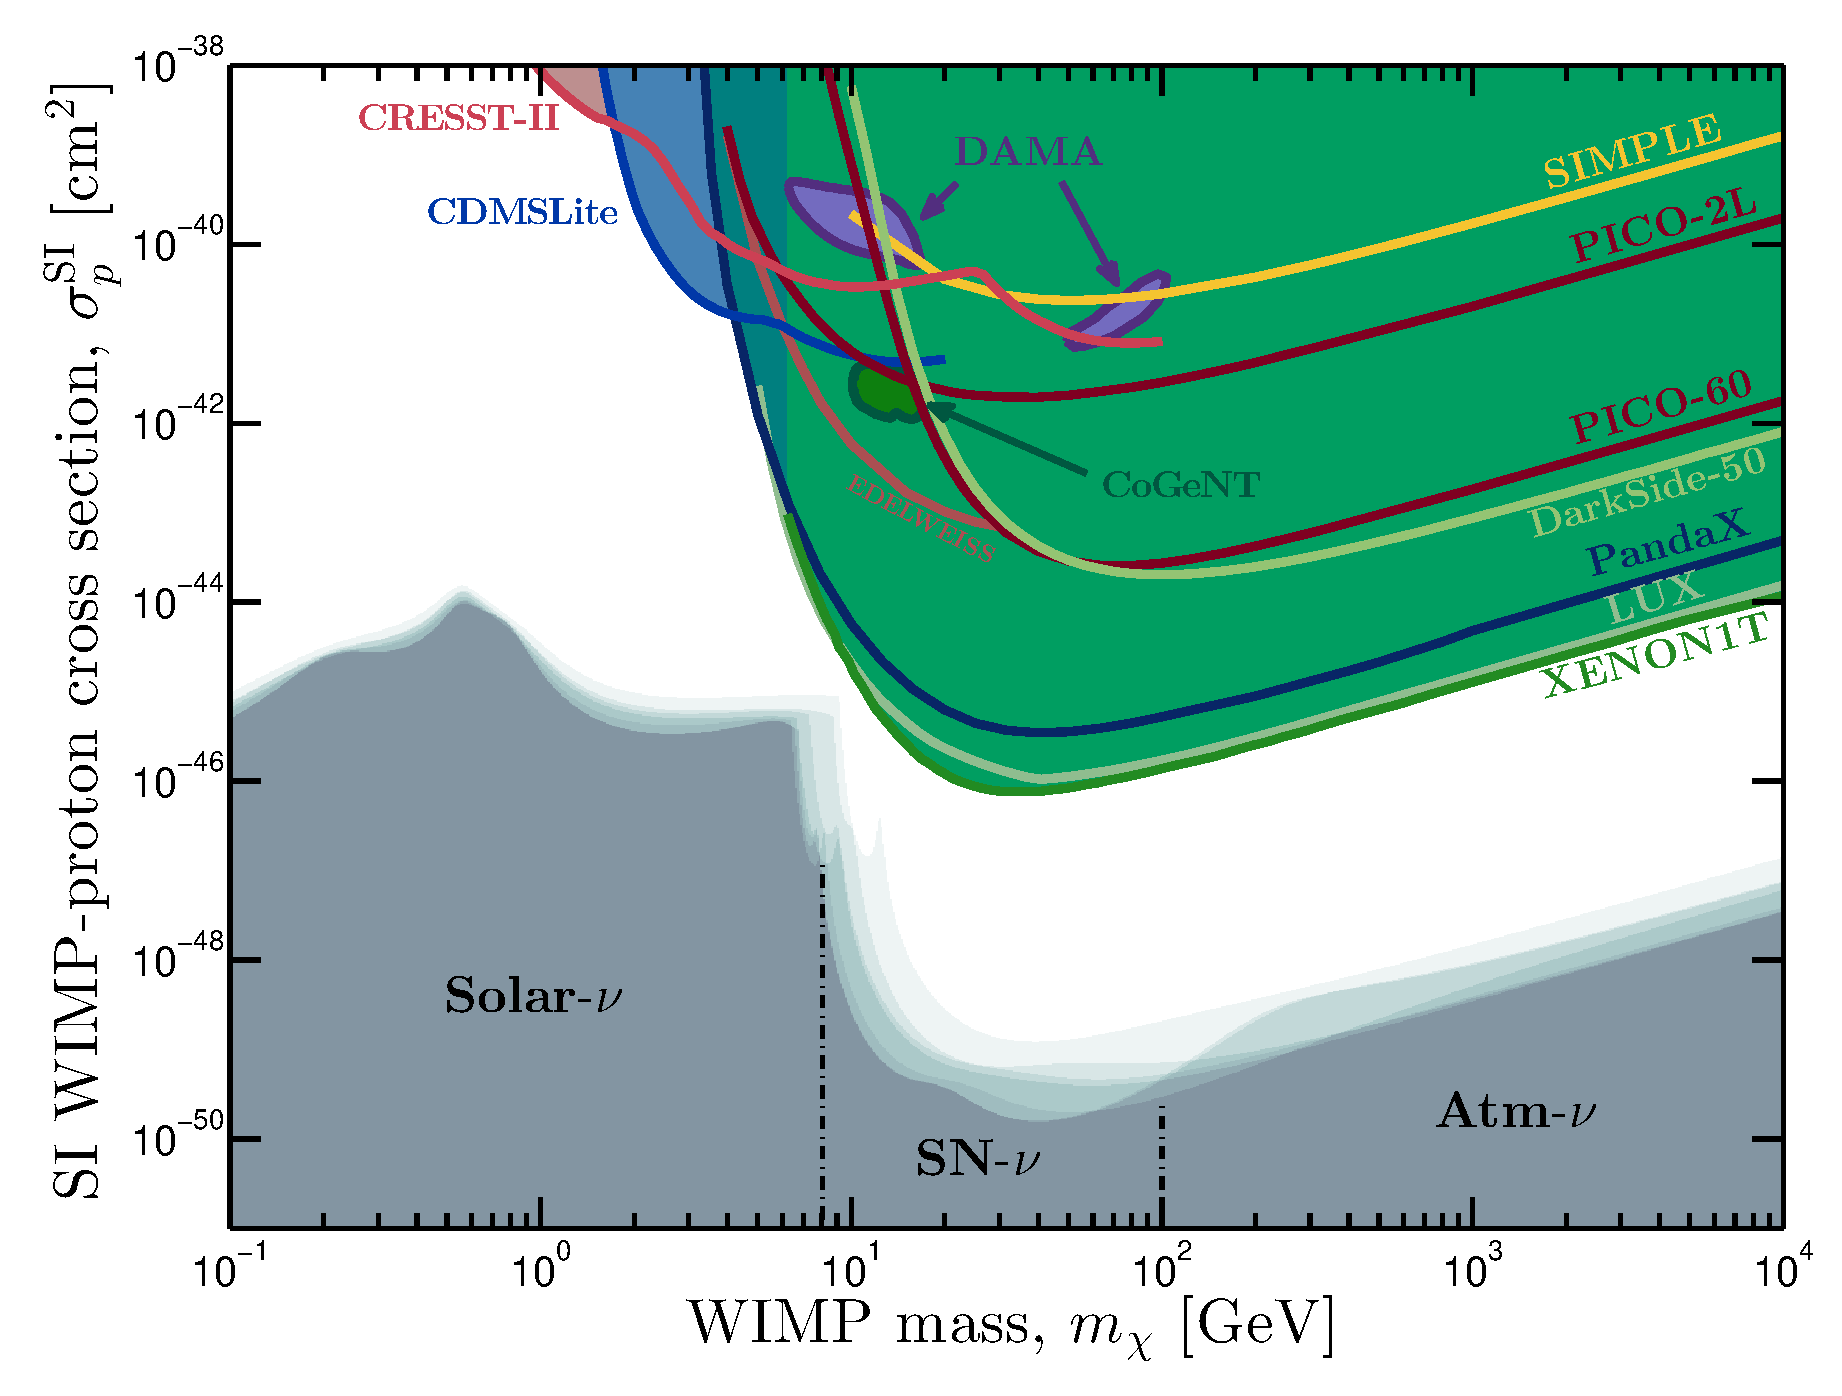
\includegraphics[width=0.9\textwidth]{Figures/WIMPlimits_SI.eps}\\
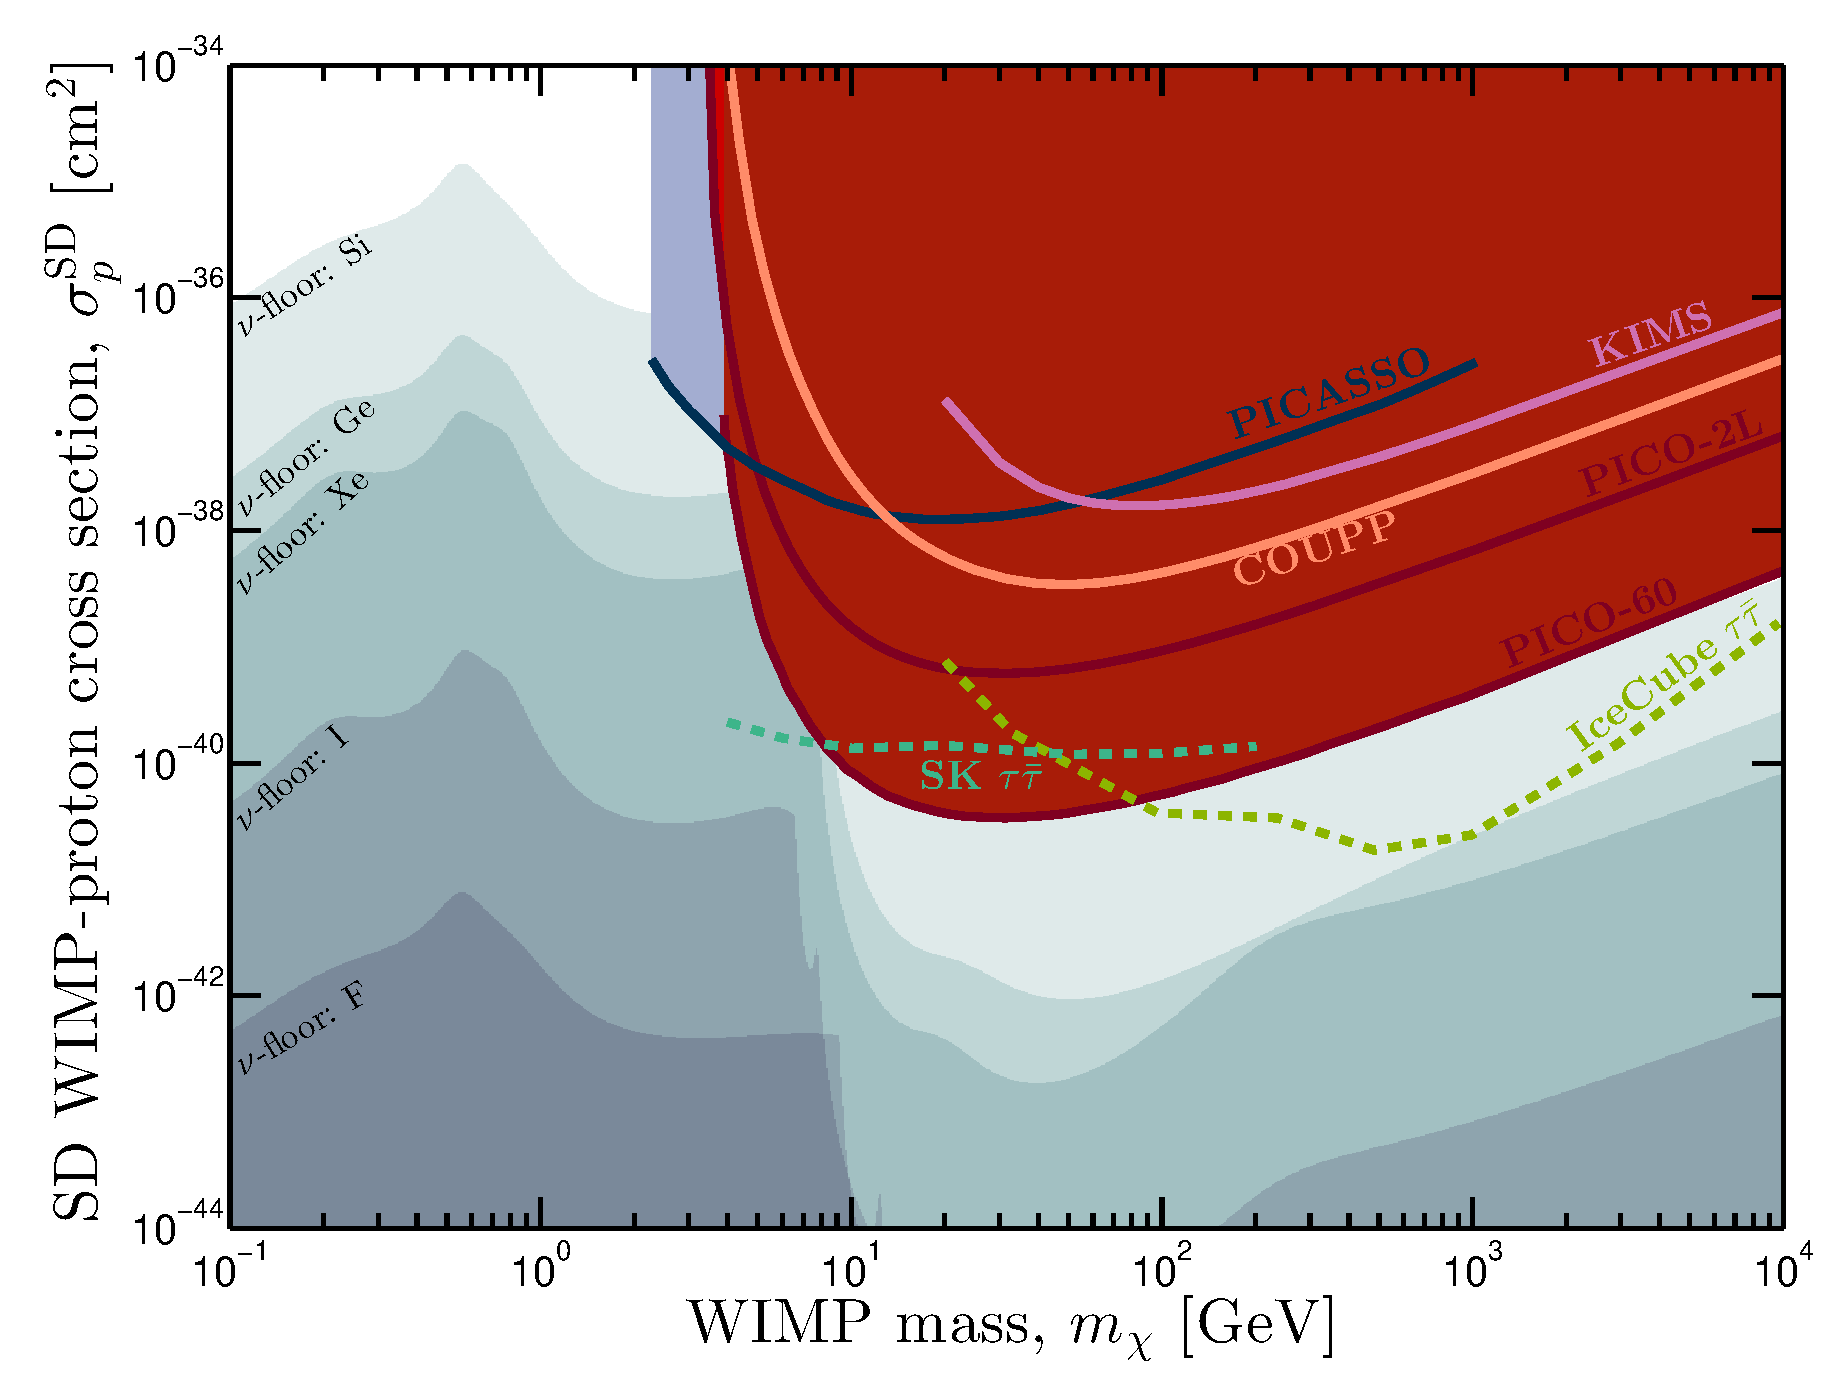
\includegraphics[width=0.9\textwidth]{Figures/WIMPlimits_SD.eps}
\caption[Current SI and SD WIMP exclusion limits]{Current excluded regions of the WIMP mass - proton cross section parameter space for spin-independent ({\bf top}) and spin-dependent ({\bf bottom}) interactions. The references for each limit are detailed in Table~\ref{tab:experiments}. The grey regions are neutrino floors for various target nuclei. In the top panel we indicate the dominant source of neutrino inducing the floor for different mass ranges: Solar neutrinos, the DSNB and atmospheric neutrinos.}\label{fig:WIMPlimits_SI}
\end{center}
\end{figure}


\begin{table}[t]\centering
\ra{1.3}
\begin{tabularx}{\textwidth}{c|YYYY}
\hline\hline
\quad		& {\bf Experiment}	& {\bf Target/Channel}	& {\bf Exposure \quad(kg days)} & {\bf Ref.} \\
\hline
\multirow{12}{*}{\bf SI:} 	& CDMSLite 		& Ge		& 70	& \cite{Agnese:2015nto}\\
				& CoGeNT	 	& Ge		& 1136	& \cite{Aalseth:2014jpa}\\
				& CRESST-II	 	& CaWO$_4$	& 52	& \cite{Angloher:2015ewa}\\
				& DAMA/LIBRA	 	& NaI		& 2.99$\times 10^6$& \cite{Savage:2008er}\\
				& DarkSide-50	 	& Ar		& 2617 & \cite{Agnes:2015ftt}\\
				& EDELWEISS	 	& Ge		& 496	& \cite{Hehn:2016nll}\\
				& LUX		 	& Xe		& 3.35$\times 10^4$& \cite{Akerib:2016vxi}\\
				& PandaX	 	& Xe		& 3.30$\times 10^4$	& \cite{Tan:2016zwf}\\
				& PICO-2L	 	& C$_3$F$_8$	& 211.5& \cite{Amole:2015lsj}\\
				& PICO-60	 	& CF$_3$I	& 3415& \cite{Amole:2015pla}\\
				& SIMPLE-II	 	& C$_2$ClF$_5$	& 30& \cite{Felizardo:2010mi}\\
				& Xenon100	 	& Xe		& 1.75$\times 10^4$& \cite{Aprile:2016swn}\\	
\hline
\multirow{5}{*}{\bf SD:} 	& COUPP		 	& CF$_3$I	& 437.4	& \cite{Behnke:2012ys}\\
				& KIMS			& CsI		& 2.45$\times 10^4$ & \cite{Kim:2012rza}\\
				& PICASSO	 	& C$_4$F$_{10}$	& 114& \cite{Archambault:2012pm}\\
				& PICO-2L	 	& C$_3$F$_8$	& 129& \cite{Amole:2016pye}\\
				& PICO-60	 	& C$_3$F$_8$	& 1167& \cite{Amole:2017dex}\\
\hline\hline
\multirow{2}{*}{$\boldsymbol{\nu}$:} 	& IceCube		 & $\chi\chi\rightarrow \tau\bar{\tau}$		& 532 days& \cite{Aartsen:2016zhm}\\
					& SK		 	& $\chi\chi\rightarrow \tau\bar{\tau}$			& 3903 days& \cite{Choi:2015ara}\\
\hline\hline
\end{tabularx}
\caption[Summary of WIMP direct detection experiments]{Summary of WIMP direct detection experiments and neutrino telescopes setting exclusion limits appearing in Fig.~\ref{fig:WIMPlimits_SI}.}
\label{tab:experiments}
\end{table}

We summarise the current status of direct detection experimental exclusion limits on both the SI and SD scattering cross sections in Fig.~\ref{fig:WIMPlimits_SI}. We list the targets, exposure and reference for each limit in Table~\ref{tab:experiments}. For the SD limits we also include the strongest indirect detection limits from neutrino telescopes IceCube and Super-Kamiokande. The limits displayed are excluded cross sections consisting of frequentist one-sided 90\% confidence intervals\footnote{Bayesian statistics are not widely used in experimental analyses but have been suggested as a means to compare multiple experiments, e.g. Ref.~\cite{Arina:2013jma}.}. There are several statistical procedures in use by different experimental collaborations to derive these exclusion limits. The choice of method depends on a number of factors relating to the knowledge of the background and the particular observables of the experiment. In cases when the underlying background can be modelled with simulations or measured with calibration data the profile likelihood ratio~\cite{Cowan:2010js} or Feldman-Cousins~\cite{Feldman:1997qc} methods are often used. For unknown or highly uncertain background conditions the maximum/optimum gap methods of Yellin~\cite{Yellin:2002xd} can be used instead which exclude cross sections based on events not appearing in certain signal intervals. In this thesis we derive limits based on mock experiments and use the profile likelihood ratio test detailed in Appendix~\ref{app:likelihood}.

The general shape of exclusion limits can be seen clearly in both panels of Fig.~\ref{fig:WIMPlimits_SI}: a sharp increase in cross section at the lowest mass extent of the limit moving towards a minimum at an intermediate mass between 10~-~100~GeV followed by a steady increase towards larger masses\footnote{Two limits in Fig.~\ref{fig:WIMPlimits_SI} deviate from this basic shape. CRESST-II has two kinks below 10 GeV which are due to the event rate transitioning between being dominated by the scattering of the three nuclei in CaWO$_4$; the kink above 10 GeV is due to the combination of the 2014 and 2015 analyses. In the CDMSLite the kink at 6 GeV is due to a particular emission line inside the detector.}. The sharp increase at low WIMP masses is due to the events from light WIMPs falling below the threshold of the experiment; lower thresholds implying smaller accessible $m_\chi$. The steady increase towards large masses is due to the decrease in the dark matter number density for heavier particles, assuming constant local density. Generally as the exposure of an experiment increases its limit will reach smaller cross sections over the full range of masses probed.

We will describe in detail the calculation of the neutrino floor in Chapter~\ref{chapter:nufloor} but we show the general appearance in the WIMP parameter space in Fig.~\ref{fig:WIMPlimits_SI}. An experiment with the naive sensitivity to reach WIMP cross sections below the grey regions will in fact have their discovery limited according to the floors shown. The shape of the floor is dependent on the energy spectrum of the WIMP signal so is dependent on target material. In the SI case this leads to only a shift by $A^2$ in cross section and a small shift in mass due to the recoil energy dependence on $m_N$. However in the SD case as well as the small shift in mass there are large differences in the cross section of the neutrino floor due to the dependence of $\mathcal{C}_{\rm SD}$ on the spin contents and isotopic fractions of the targets. For elements such as Si for example the isotopic fraction of the spin possessing isotope is very small, inducing a large upward shift in the regime of cross sections which produce similar event rates to the neutrino backgrounds. 

\subsection{Future experiments}\label{sec:direct_future}
Many of the experiments mentioned in the previous section are being upgraded or are merging with other collaborations. XMASS2~\cite{Hiraide:2015cba}, DEAP-3600~\cite{Boulay:2012hq}, Xenon1T/nT~\cite{Aprile:2015uzo}, DarkSide~\cite{Aalseth:2015mba} are planned or in construction upgrades to existing experiments. In addition, new collaborations have formed in recent years such as LZ~\cite{Akerib:2015cja}, EURECA~\cite{Angloher:2014bua} as well as DARWIN the proposed multi-ton xenon detector~\cite{Aalbers:2016jon}. This `next generation' of ton-scale detector are expected to be the first to detect coherent neutrino-nucleus scattering and reach the neutrino floor.

In addition to the tried and tested methods for rare event detection, the literature contains a wealth of alternative ideas which rely on upcoming or far-future technology. Some of these ideas are pointed particularly towards the light WIMP regime ($<$10~GeV) where much of the parameter space remains unexplored. New ideas such as the use of CCD chips in the DAMIC experiment~\cite{Barreto:2011zu} or experiments using $^4$He~\cite{Guo:2013dt} involve light targets so are ideal for low mass searches. However arguably the most powerful signal that one would hope to exploit in the future is directionality and there is considerable effort in constructing detectors that can measure recoil track directions. It may also be possible to adapt existing experimental technology in some directionally sensitive extension. We explore directional detection in detail in the next Chapter.

\section{Summary}\label{sec:direct_summary}
In this Chapter we have detailed the theoretical and experimental factors required for calculating signals in present and future direct detection experiments. We first discussed the ingredients from particle physics which predict spin-independent and spin-dependent event rates. We also outlined the astrophysical input from the local phase space distribution of dark matter in the Milky Way. We concluded with a discussion of the current status of the experimental direct detection effort with a summary of the various exclusion limits made on the WIMP cross section-mass parameter space. Now that we have established the status of direct detection the following Chapters will be forward-looking, exploring the future strategies we must employ to solve some of the problems we have already touched upon. We begin with directional detection experiments and how they may allow us to measure the dark matter distribution around us. We then look at how the neutrino floor will impact upcoming ton-scale experiments and describe how directional detectors will be required to overcome it.